\newpage
\section{Boundary Value Problem for the Heat Equation}

\subsection{Properties of the heat equation}
Consider the heat equation in $\mathbb{R}^{+} \times \mathbb{R}^{n}$.
$$
\left\{\begin{array}{l}
\left(\partial_{t}-\Delta\right) u=f \\
u(0)=u_{0}
\end{array}\right.
$$
We have already seen how to derive a solution via the fundamental solution:
$$
u=f *_{x, t} K(t)+u_{0} *_{x} K(t), \quad K(t)=\frac{1}{(4 \pi t)^{n / 2}} e^{-x^{2} /(4 t)} \mathbb{1}_{\{t \geq 0\}}
$$
This is the unique solution going forward in time which is a temperate distribution.

Here are some key properties for the homogeneous equation given by this fundamental solution: Consider the heat equation in $\mathbb{R}^{+} \times \mathbb{R}^{n}$.
$$
\left\{\begin{array}{l}
\left(\partial_{t}-\Delta\right) u=0 \\
u(0)=u_{0}
\end{array}\right.
$$

\begin{itemize}
    \item Infinite speed of propagation: Even if $u_{0}$ has compact support, the solution $u$ immediately spreads to all of $\mathbb{R}^{n}$.
    \item Instant regularization:
    $$
    u(t)=K(t) * u_{0}
    $$
    where $K(t)$ is smooth for $t>0$. So $u$ is smooth for $t>0$.
    \item The fundamental solution has Gaussian decay at $\infty:$ This means that any initial data $u_{0}$ with $\left|u_{0}\right| \leq e^{c x^{2}}$ will generate a local in time solution.
\end{itemize}

\subsection{The mean value property and the maximum principle}
Now let's look at the heat equation in a domain $\Omega \subseteq \mathbb{R}^{n}$.
$$
\begin{cases}\left(\partial_{t}-\Delta\right) u=f & \text { in } \Omega \times \mathbb{R}^{+} \\ u(t=0)=u_{0} & \text { in } \Omega \\ u(t, x)=g & \text { on } \partial \Omega \times \mathbb{R}^{+}\end{cases}
$$
The third equation is a \textbf{Dirichlet boundary condition}. We could replace it with a \textbf{Neumann boundary condition}
$$
\frac{\partial u}{\partial \nu}(t, x)=g \quad \text { on } \partial \Omega \times \mathbb{R}^{+}
$$

As with the Laplace equation, we use either one boundary condition or the other but not both.

Here are several ways to approach this:
\begin{itemize}
    \item Via a maximum principle.
    \item Via energy estimates.
    \item Using Green's functions.
\end{itemize}
We first discuss the maximum principle. First, is there a mean value property for the heat equation? We would like to write something like
$$
u\left(t_{0}, x_{0}\right)=\frac{1}{|D|} \int_{D} u(t, x) dt d x
$$
for some $D$. For the Laplace equation, we used a ball for $D$, but this should not be the case for the heat equation; unlike for the Laplace equation, balls are not level sets of the fundamental solution. We may also ask if we need any weights for the maximum principle.

Step 1: Green's theorem for the heat equation: Let $u,v$ be such that $v$ has compact support. Then 
$$
\iint\left(\partial_{t}-\Delta\right) u \cdot v d x d t=\iint\left(-\partial_{t}-\Delta\right) v \cdot u d x d t
$$
If we want to get $u(0,0)$ out of the right hand side, then we would need $\left(-\partial_{t}-\Delta\right) v=\delta_{(0,0)}$. Here, $-\partial_{t}-\Delta$ is the adjoint heat operator, which is a "backward heat operator" and gives a backward heat equation with a fundamental solution
\[
    K^{\text {back }}(x, t)=-\frac{1}{(4 \pi|t|)^{n / 2}} e^{x^{2} /(-4 t)} 1_{\{t \leq 0\}}
\]
Define the parabolic balls
$$
D_{r}(0,0)=\left\{\left|K^{\text {back }}(x, t)\right| \ge r^{-n}\right\}
$$
What do these sets look like? If $x=0$, then $K \asymp t^{-n / 2}$, and $t^{-n / 2} \geq r^{-n}$ iff $|t| \leq r^{2}$. To figure out the sideways boundaries of these regions, take $t \approx -\frac{1}{2} r^{2}$. Now change $x$ so that $e^{x^{2} /(4 t)} \gtrsim 1$. Then $|x| \leq \sqrt{-t} \approx r$. This looks like an ellipse, but near $(0,0)$, there is a logarithmic coorection to a parabola.

\begin{figure}[H]
    \centering
    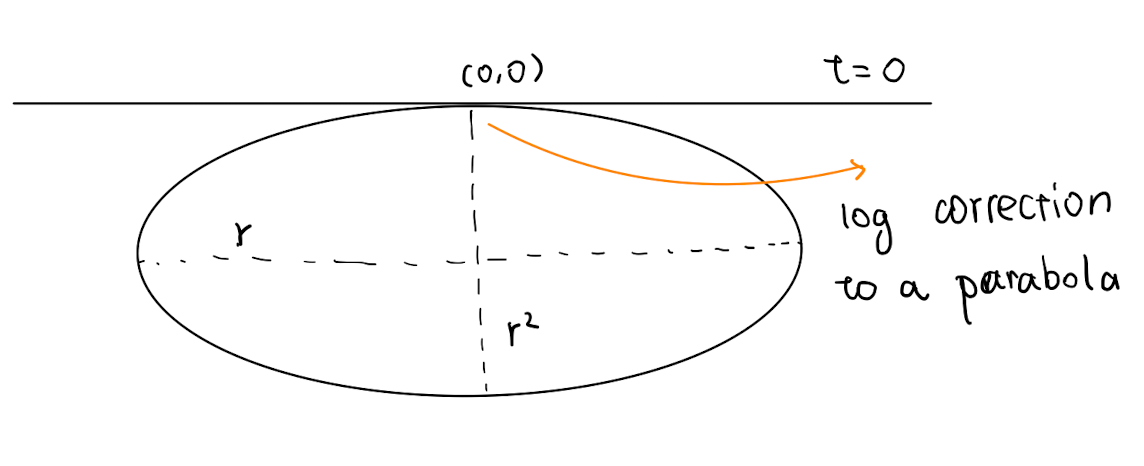
\includegraphics[width=0.5\textwidth]{Pics/24-1.png}
\end{figure}

Our goal is to show that
$$
u(0,0)=\int_{D_{r}(0,0)} \omega(t, x) u(t, x) d x
$$
for some suitable positive weight $\omega$ (we want positive so we can think of this as an average). Look at our Green's theorem in $D_{r}(0,0)$, which gives boundary terms:
$$
\begin{aligned}
\iint_{D_{r}(0,0)}\left(\partial_{t}-\Delta\right) u \cdot v d x d t=\iint_{D_{r}(0,0)}\left(-\partial_{t}-\Delta\right) v \cdot u d x d t & \\
+& \int_{\partial D_{r}(0,0)} \nu_{t} \cdot u v-\frac{\partial u}{\partial \nu} \cdot v+u \cdot \frac{\partial v}{\partial \nu} d \sigma
\end{aligned}
$$
For $v=K^{\text {back }}(t, x)$, this does not work because we get boundary terms. Instead, we can try
$$
v=K^{\mathrm{back}}(t, x)+r^{-n}
$$
which makes $v=0$ on $\partial D_{r}(0,0)$. This makes the first two boundary terms equal 0 , but we would also like to make sure that $\frac{\partial v}{\partial \nu}=0$ on $\partial D_{r}(0,0)$. This is the same as saying that $\nabla v=0$ on $\partial D_{r}$. The way we can alter our fundamental solution to take advantage of this is
$$
v=K^{\mathrm{back}}(t, x)+r^{-n}+c \ln \left(-K^{\mathrm{back}} \cdot r^{n}\right)
$$
where $c$ is chosen so that $\nabla v=0$ on $\partial D_{r}(0,0)$. This choice gives us
$$
\begin{aligned}
\nabla v &=\nabla K+c \frac{\nabla K}{K} \\
&=\nabla K\left(1+\frac{c}{K}\right)
\end{aligned}
$$
and since $K=-r^{n}$ on the boundary, we can pick $c=r^{n}$.
If $\left(\partial_{t}-\Delta\right) u=0$, then we get
$$
\iint D_{t}(-\partial-\Delta) v \cdot u d x d t=0
$$
We can calculate
$$
\begin{aligned}
\left(-\partial_{t}-\Delta\right) v &=\delta_{(0,0)}+c\left(-\partial_{t}-\Delta\right) \ln \left(-r^{n} K^{\mathrm{back}}\right) \\
&=\delta_{(0,0)}-c \frac{\partial_{t} K^{\mathrm{back}}}{K^{\mathrm{back}}}-c \nabla \cdot \frac{\nabla K^{\mathrm{back}}}{K^{\mathrm{back}}} \\
&=\delta_{(0,0)}-c \underbrace{\frac{\left(\partial_{t}-\Delta\right) K^{\mathrm{back}}}{K^{\mathrm{back}}}}_{=0}+c \frac{\left(\nabla K^{\mathrm{back}}\right)^{2}}{\left(K^{\mathrm{back}}\right)^{2}} \\
&=\delta_{(0,0)}+c\left(\nabla \ln K^{\mathrm{back}}\right)^{2}
\end{aligned}
$$
where this is a spatial gradient.
$$
=\delta_{(0,0)}-r^{-n} \frac{x^{2}}{4 t^{2}}
$$
We get:

\begin{theorem}
    [Mean value property]
    If $\left(\partial_{t}-\Delta\right) u=0$ in $\Omega \times[0, T]$,
$$
u(0,0)=r^{-n} \int_{D_{r}(0,0)} \frac{x^{2}}{4 t^{2}} u(t, x) d x d t
$$
\end{theorem}
\begin{remark}
    How do we know this is an average? This holds for all solutions to the heat equation, so plug in a constant. This gives
$$
r^{-n} \int_{D_{r}(0,0)} \frac{x^{2}}{4 t} d x d t=1
$$
So this is indeed a weighted average.
\end{remark}

For our maximum principle, what is the boundary of our region $C_T = \bar \Omega \times [0,T]$?

\begin{figure}[H]
    \centering
    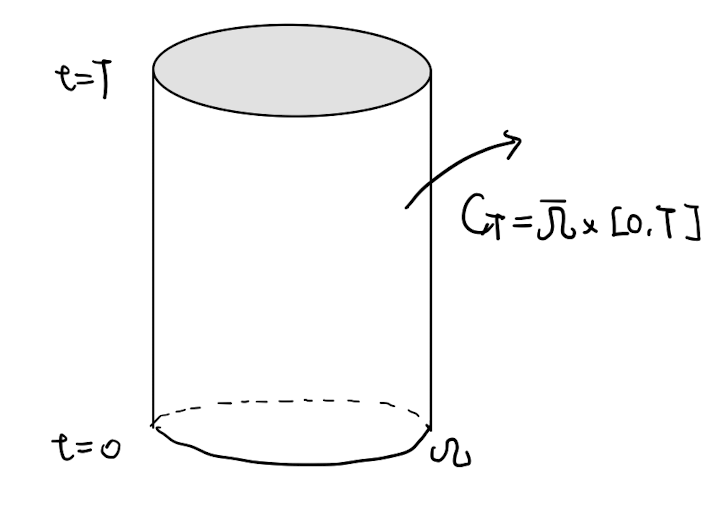
\includegraphics[width=0.3\textwidth]{Pics/24-2.png}
\end{figure}

If you consider causality, the $t=T$ boundary is determined by the rest, so it should not be considered. Write $\partial C_{T}=\bar{\Omega} \times\{0\} \cup \partial \Omega \times[0, T] .$ The first part is the bottom, and the second part is the lateral boundary. Together, they make up the parabolic boundary of $C_{T}$.

\begin{theorem}
[Strong maximum principle]
If $\left(\partial_{t}-\Delta\right) u=0$ in $\Omega \times[0, T]$, then 
$$
\max _{C_{T}} u=\max _{\partial C_{T}} u.
$$

Further if $u\left(t_{0}, x_{0}\right)=\max u$ for some $\left(t_{0}, x_{0}\right)$ inside, then $u$ is constant for $t \leq t_{0}.$
\end{theorem}
\begin{proof}
    Take $\left(t_{0}, x_{0}\right)$ to be a maximum inside. Then the mean value property gives
    $$
    \begin{aligned}
    \max u &=u\left(t_{0}, x_{0}\right) \\
    &=r^{-n} \int \frac{\left(x-x_{0}\right)^{2}}{(t-t-0)^{2}} u(t, x) d x d t \\
    & \leq r^{-n} \int \frac{\left(x-x_{0}\right)^{2}}{(t-t-0)^{2}} \max u d x d t \\
    &=\max u
    \end{aligned}
    $$
    Equality must hold, so $u=\max u$ in $D_r(t_0, x_0)$.
    \begin{figure}[H]
        \centering
        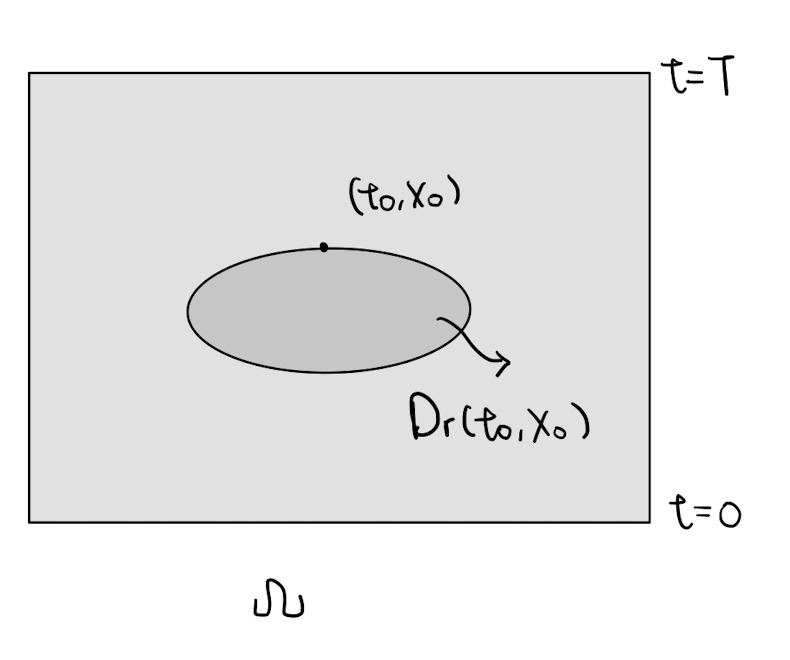
\includegraphics[width=0.5\textwidth]{pics/24-3.png}
\end{figure}
How do we get the whole region ${t\le t_0}$? Here is a picture: 
\begin{figure}[H]
    \centering
    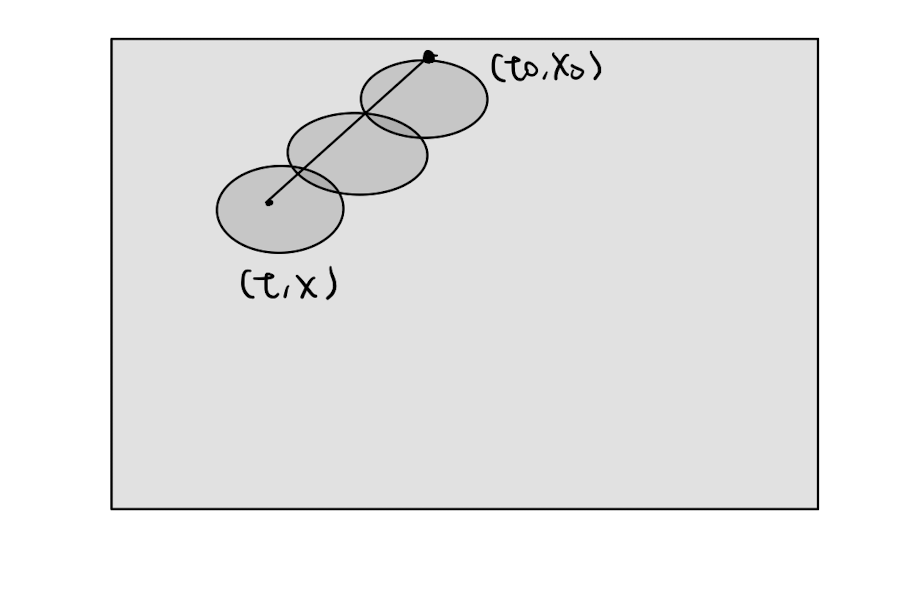
\includegraphics[width=0.5\textwidth]{pics/24-4.png}
\end{figure}
\qed 
\end{proof}

\begin{remark}
    Just like with the Laplace equation, we can talk about subsolutions
    $$
    \left(\partial_{t}-\Delta\right) u \leq 0
    $$
    and supersolutions
    $$
    \left(\partial_{t}-\Delta\right) u \geq 0
    $$
    Using the mean value property with inequalities gives a maximum principle for subsolutions and a minimum principle for super solutions.
\end{remark}

\begin{theorem}
    [Comparison principle]
     Let $u^{-}$be a subsolution and $u^{+}$be a supersolution for the heat equation. If $u^{-} \leq u^{+}$on $\partial C_{T}$, then $u^{-} \leq u^{+}$in $C_{T}$.
\end{theorem}

\begin{corollary}
    The solution to the bounded heat equation is unique.
\end{corollary}

\subsection{Energy estimates}
Consider the homogeneous Dirichlet problem
$$
\left\{\begin{array}{l}
\left(\partial_{t}-\Delta\right) u=0 \quad \text { in } \Omega \times[0, T) \\
u(0)=u_{0} \\
u(\partial \Omega)=0
\end{array}\right.
$$
and let
$$
E(u(t))=\int|u(t, x)|^{2} d x
$$
Then we can compute
$$
\begin{aligned}
\frac{\partial}{\partial t} E(u(t)) &=2 \int u \cdot u_{t} d x \\
&=2 \int u \cdot \Delta u d x\\
&= -2\int |\nabla u|^2 \,dx\\
&\le 0,
\end{aligned}
$$
which tells us that $E$ is nonincreasing in time $E(t) \leq E(0) .$ So if $u_{0}=0$, then $E(t)=0$, which gives $u(t)=0$.
We can also look at the relation
$$
\|u(0)\|_{L^{2}}^{2}=\|u(T)\|_{L^{2}}^{2}+\int_{0}^{t}|\nabla u|_{L^{2}}^{2} d x
$$
If we start with $u(0) \in L^{2}$, we get $ u(T) \in L^{2}$ for a.e. $T$. We can think of this as a \textbf{parabolic regularizing effect}.